\chapter{Background}

% A more extensive coverage of what's required to understand your
% work. In general you should assume the reader has a good undergraduate
% degree in computer science, but is not necessarily an expert in
% the particular area you've been working on. Hence this chapter
% may need to summarize some ``text book'' material.

% This is not something you'd normally require in an academic paper,
% and it may not be appropriate for your particular circumstances.
% Indeed, in some cases it's possible to cover all of the ``background''
% material either in the introduction or at appropriate places in
% the rest of the dissertation.

This chapter reviews background relevant to the remainder of this dissertaion.
The scope includes an overview of music theory and automatic composition
and also includes coverage of sequence probability models.

\section{A primer on Western music theory}

Music theory is a branch of musicology concerned with the study of the rules
and practices of music. While the general field includes study of acoustic
qualities such as timbre and waveform synthesis, our work is concerned with
modelling the musical composition itself rather than acoustic features. This is
justified because acoustic features are more closely related to a particular
reproduction (e.g. the skill of the performers, quality of the instruments) and
are likely to vary significantly across different performances. Indeed,
references to a piece of music generally refer to the underlying composition
itself rather than any particular performance of the piece. This suggests that
the composition itself is more significant and hence a more desirable modeling
target.

\subsection{Pitches, durations, and notes: the basic building blocks}

A \emph{note} is the most fundamental element of music and possesses two
primary attributes, a \emph{pitch} and a \emph{duration}. Though pitch is
closely related to physical frequency of vibration of a waveform (as measured
in Hertz), pitch its a perceptual property whose semantic meaning is derived
from a listener's perception. This distinction has been scrutinized by Terhardt
\cite{:/content/asa/journal/jasa/55/5/10.1121/1.1914648}, whose visual analogy
in \autoref{fig:pitch} illustrates how a pitch can be heard even if its
percieved frequency is absent just as one may see the word ``PITCH'' despite
being presented with only a suggestive shadow.

\begin{figure}[htpb]
    \centering
    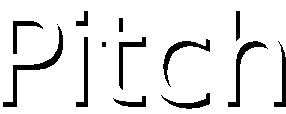
\includegraphics[width=0.6\linewidth]{Figures/pitch.pdf}
    \caption{Terhardt's visual analogy for pitch. Similar to how
        the viewer of this figure may percieve contours not present, pitch
        describes subjective information received by the listener even when
    physical frequencies are absent.}
    \label{fig:pitch}
\end{figure}

Despite its psychoacoustic nature, it is nevertheless useful to objectively
quantify pitch as a frequency. To do so, we first need some definitions. The
difference between two frequencies is called an \emph{interval} and an
\emph{octave} is an interval corresponding to the distance between a frequency
$f \in \RR^+$ and its doubling $2f$ or halving $f/2$. Two frequencies spaced
exactly an octave apart are perceived to be similar, suggesting that music is
percieved on a logarithmic scale.

Most Western music is based on the \emph{twelve-note chromatic scale}, which
divides an \emph{octave} into twelve distinct frequencies. The \emph{tuning
system} employed dictates the precise intervals between subdivisions, with
\emph{equal temperament tuning} (all subdivisions are equally spaced on a
logarithmic scale) presently the most widely used
method\cite{denton1997history}. \todo{Talk about well-tempered tuning and bach}
Under twelve-note equal temperament tuning, the distance between two
consecutive subdivisions ($1/12$ of an octave) is called a \emph{semitone}
(British) or \emph{half-step} (North American) and two semitones constitutes
a \emph{tone} or \emph{whole-step}.

When discussing music, \emph{note names} which enable succinct specification of
a musical pitch are often employed. In \emph{scientific pitch notation},
\emph{pitch classes} which represent a pitch modulo the octave are specified by
a letter ($C, D, E, F, G, A, B$) and optionally a single \emph{accidental}. Pitch
classes without accidentals are called \emph{natural} and correspond to the white
keys on a piano. Two accidentals are possible: sharps ($\#$) raise the natural
pitch class up one semitone and flats ($\flat$) lower by one semitone.
\autoref{fig:piano-keys} illustrates how these pitch classes map to keys on a
piano.

\begin{figure}[htpb]
    \centering
    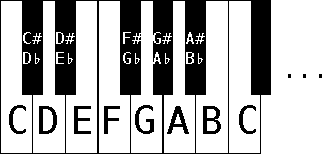
\includegraphics[width=0.6\linewidth]{Figures/piano-keys.pdf}
    \caption{Illustration of an octave in the 12-note chromatic scale
        on a piano keyboard.}
    \label{fig:piano-keys}
\end{figure}

Since pitch classes represent equivalence class of frequencies spaced an
integral number of octaves apart, unambiguously specifying a pitch requires not
only a pitch class but also an octave. In scientific pitch notation, this is
accomplished by appending an octave number to a pitch class letter (see
\autoref{fig:pitch-class}). Together, a pitch class and octave number uniquely
specify the notation for a pitch. On sheet music, the pitch of a note is
indicated by its vertical position with respect to the \emph{stave} (the five
horizontal lines and four spaces).

\begin{figure}[htpb]
    \centering
    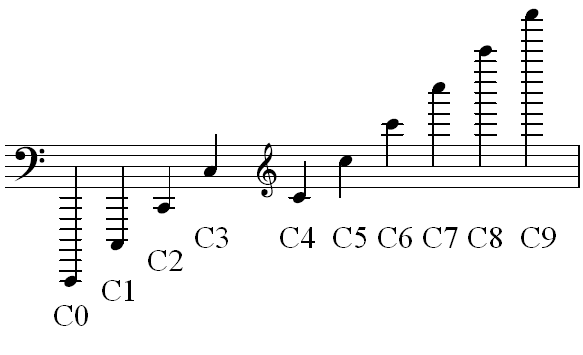
\includegraphics[width=0.6\linewidth]{Figures/Pitch_notation.png}
    \caption{Scientific pitch notation and sheet music notation of $C$ notes at
    ten different octaves.  \todo{Cite wiki scientific pitch notation}}
    \label{fig:pitch-class}
\end{figure}

Note that the discussion of pitch thus far has not made any direct connection
between pitch and frequency. Indeed, this lack of dependence on absolute
physical frequency highlights music's \emph{transposition invariance property}:
many semantically relevant features in music are present the relative relations
between pitches rather than absolute frequencies and hence remain invariant
when the entire piece of music is offset by a constant frequency. However, a
fixed reference frequency is oftentimes required for performance and
reproduction purposes. To convert from pitch notation to physical frequencies,
common modern practice is to tune $A4$ to 440 Hz (a practice known as A440).

In addition to pitch, a note also possesses a \emph{duration}. The duration of
a note indicates how long it is to be played and is measured in fractions of a
\emph{whole note} (American) or \emph{semibreve} (British). Perhaps the most
common duration is a \emph{quarter-note} (American) or \emph{crotchet}
(British). Other note durations are also possible and the most common along
with their notation in sheet music are enumerated in
\autoref{fig:note-durations}. The relationship between durations and
physical time intervals is given by the \emph{tempo}, which is usually
denoted near the start of the piece in beats per minute.

\begin{figure}[htpb]
    \centering
    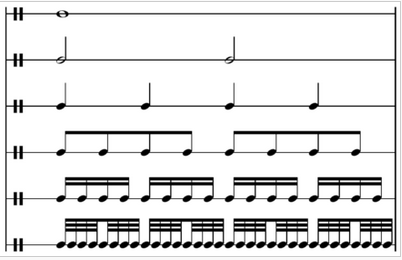
\includegraphics[width=0.6\linewidth]{Figures/note-durations.png}
    \caption{Comparison of various note durations. \todo{Cite wiki Whole note}}
    \label{fig:note-durations}
\end{figure}

Our work focuses in particular on \emph{tonal music}, a genre of music
characterized by the prevalence of one pitch class (the \emph{tonic}) around
which the melody and harmony are built.

A basic concept within tonal music is the \emph{scale}, which defines a subset
of pitch classes that are ``in key'' with respect to the tonic. Two fundamental
scales are the major (with step pattern
whole-whole-half-whole-whole-whole-half) and minor scales
(whole-half-whole-whole-half-whole-whole). The choice of tonic and scale is
collectively referred to as the \emph{key}. Many musical phenomena such as
stability, mood, expectation, and resolution can be attributed to choice of key
and \emph{modulations} (i.e. changes in key during the middle of a piece of
music).

\section{Neural sequence probability modeling}

Our work in later sections make heavy use of neural networks. In this section,
we briefly review the relevant concepts and set up notation.

\subsection{Neurons: the basic computation unit}

Neurons are the basic abstraction which are combined together to form
neural networks. A \emph{neuron} is a parametric model of a function $f : \RR^D \to
\RR$ from its $D$-dimensional input $\x$ to its output $y$. Our neurons will be
defined as
\begin{equation}
    f(\x) \coloneqq \sigma( \langle \vec{w}, \x \rangle)
\end{equation}
which can be viewed as an inner product with \emph{weights} $\vec{w}$ to
produce an \emph{activation} $z \coloneqq \langle \vec{w}, \x \rangle
\in \RR$ which is then squashed to a bounded domain by a non-linear
\textbf{activation function} $\sigma : \RR \to [L, U]$. This is visually
depicted in \autoref{fig:nn-single}, which also makes apparent the
interpretation of weight $w_i$ as the sensitivity of the output $y$ to the
input $x_i$.

\begin{figure}[htpb]
    \centering
    \input{Figures/nn-single.pdf_tex}
    \caption{A single neuron first computes an activation $z$ and then passes it through
    an activation function $\sigma(\cdot)$}
    \label{fig:nn-single}
\end{figure}

\subsection{Feedforward neural networks}

Multiple neurons may share inputs and have their outputs concatenated together
to form a \emph{layer} modelling a multivariate functions $f :
\RR^{D_\text{in}} \to \RR^{D_\text{out}}$. Multiple layers can then
be composed together to form a \emph{feedforwd neural network}.

\begin{figure}[htpb]
    \centering
    \input{Figures/nn-ffw.pdf_tex}
    \caption{Graph depiction of a feedforward neural network with $2$ hidden layers}
    \label{fig:nn-ffw}
\end{figure}

Although a single hidden layer is theoretically sufficient for a universal
function approximator\cite{Cybenko1993}, the number of hidden units to
guarantee reported theoretical bounds are usually unfeasibly large. Instead,
recent work in \emph{deep learning} has shown that deep models which contain
many hidden layers can achieve strong performance across a variety of
tasks\cite{Bengio2011}.

The improved modeling capacity gained by composing multiple layers is due to
the composition of multiple non-linear activation functions.
In fact, it is easy to show that removing activation functions would make
a deep network equivalent to a single matrix transform: let $\W_{l,l+1}$
denote the weights between layers $l$ and $l+1$. The original neural network
computes the function
\begin{equation}
    \sigma\left(
        \W_{L,L-1} \sigma \left(
            \W_{L-1,L-2}\cdots \sigma \left(
                \W_{2,1} \x
            \right) \cdots
        \right)
    \right)
\end{equation}
After removing the activation functions $\sigma$, we are left with
\begin{equation}
    \W_{L,L-1} \W_{L-1,L-2}\cdots \W_{2,1} \x
    = \x
    = \tilde{\W} \x
\end{equation}
where $\tilde{\W} = \left(\prod_{i=1}^{L-1} \W_{i,i+1} \right)$
is a matrix transform computing the same function as the neural network with
activation functions removed.

\subsection{Recurrent neural networks}

While feedforward neural networks provide a flexible model for approximating
arbitrary functions, they require a fixed-dimension input $\x$ and hence
cannot be directly applied to sequential data $\x = (x_t)_{t=1}^T$ where $T$ may
vary.

\todo{Introduce $\theta$ for parameters}

A naive method for extending feedforward networks would be to independently
apply a feedforward network to compute $y_t = f(x_t; \theta)$ at each timestep
$1 \leq t \leq T$. However, this approach is only correct when each output $y_t$
only depends on the input at the current time $x_t$. This assumption
is false in many scenarios: the current musical note depends on the sequence of
notes leading up to it.

This shortcoming motivates \emph{recurrent neural networks} (RNNs), which
generalize feedforward networks by introducing time-delayed recurrent
connections between hidden layers (Elman networks \cite{elman1990finding}) or
from the output layers to the hidden layers (Jordan networks
\cite{jordan1997serial}). \autoref{fig:nn-rnn} illustrates an Elman-type network:
note that apart from the edges between hidden nodes, the network is identical to
a standard network (\autoref{fig:nn-ffw}).

\todo{Why do we use Elman}

\begin{figure}[htpb]
    \centering
    \input{Figures/nn-rnn.pdf_tex}
    \caption{Graph depiction of an Elman-type RNN. Note the recurrent connections
    within the hidden layer.}
    \label{fig:nn-rnn}
\end{figure}

\autoref{fig:rnn-elman} reinterprets the recurrent hidden layer connections in
\autoref{fig:nn-rnn} as inputs whose values are taken from the previous hidden
state making the time-delay explicit. Additionally, \autoref{fig:rnn-elman}
introduces the notion of \emph{memory cells}, which abstract the internals
of RNNs into a computational unit which for each timestep $t$:
\begin{itemize}
    \item Takes as inputs
        \begin{itemize}
            \item The current element in the input sequence $\x_t$
            \item The previous hidden state $\h_{t-1}$
        \end{itemize}
    \item Produces the outputs
        \begin{itemize}
            \item The updated hidden state $\h_t = f_h (\x_t, \h_{t-1})$
            \item The outputs $\y_t = f_y (\h_t)$.
        \end{itemize}
\end{itemize}

\begin{figure}[htpb]
    \centering
    \input{Figures/nn-rnn-elman.pdf_tex}
    \caption{Equivalent formulation of an Elman-type RNN treating the time-delayed hidden state
    as additional inputs to a feedforward network}
    \label{fig:rnn-elman}
\end{figure}

The memory cell abstraction is convenient because it enables discussion of RNN
architecture without settling on a particular memory cell implementation. In
particular, it enables us to \emph{unroll the RNN} by removing the time-delayed
recurrent cycle and replicating the memory cell over multiple timesteps as seen
in \autoref{fig:rnn-single-unrolled}. This gives rise to a finite directed
acyclic graph where nodes represent pieces of data and edges $s \to t$ indicate
that $t$ is a function of $s$.

It is interesting to note the similarity between unrolled RNN and feedforward
networks: both are acyclic and the semantic meaning of the nodes and edges are
identical. In fact, one can view an unrolled RNN as a feedforward network with
as many layers as the elements in the input sequence $(\x_t)_t$ and
parameters tied across all layers. This similarity has inspired fruitful
cross-polination in both fields: methods for training feedforward networks have
been adapted to RNNs and methods for learning long timespan dependencies in
RNNs have been used to train even deeper neural networks. \todo{Foreshadow, or
use as a transition}. \todo{Depth in time makes training difficult, similar to
    DNNs. LSTM inspires highway networks for DNNs DNNs and grid-LSTMs for deep
LSTMs}

\begin{figure}[htpb]
    \centering
    \input{Figures/rnn-single-unrolled.pdf_tex}
    \caption{Signal flow diagram representation of a single-layer RNN and its corresponding
    expansion into a computation graph}
    \label{fig:rnn-single-unrolled}
\end{figure}

\autoref{fig:rnn-single-unrolled} makes it obvious how the hidden state is
carried along throughout the sequence of computations, giving rise to a useful
alternative interpretation of the hidden state as a temporal memory mechanism.
Under this interpretation, we can view the hidden state update $\h_t = f_h
(\x_t, \h_{t-1})$ as \emph{writing} information extracted from the
current inputs $\x_t$ to the memory $\h_{t-1}$. Similarly, producing
the outputs $\y_t = f_y (\h_t)$ can be seen as \emph{reading}
information from the hidden state.

\todo{Compare to N-grams; show how it's like an infinite context. One
    interpretation is to view the hidden state $\h_t$ as an
    infinite-length prior context window, summarizing all of the prior inputs
    into into a compact fixed-size vector.}

Since the RNN outputs $\y$ also form a sequence with the same length as
the inputs $\x$, they can be used as inputs into another RNN. This
stacking of multiple memory cells is similar to the layering seen in deep
neural networks, giving rise to the term \emph{deep neural sequence models}
\todo{Cite?}. This is illustrated in \autoref{fig:rnn-multi-unrolled}.

\begin{figure}[htpb]
    \centering
    \input{Figures/rnn-multi-unrolled.pdf_tex}
    \caption{Unrolled computation graph for a 2-layer RNN}
    \label{fig:rnn-multi-unrolled}
\end{figure}

The greater modeling capabilities of multilayer RNNs can be attributed to two
primary factors: composition of multiple non-linearities and an increase in the
number of paths through which information can flow. The former is analogous to
the feedforward case: stacking memory cells increases the number of
non-linearities in the composite cell just like stacking multiple layers in
feedforward networks. To understand the latter point, notice that in
\autoref{fig:rnn-single-unrolled} there is only a single path from
$\x_{t-1}$ to $\y_{t}$ hence the conditional independence
$\y_{t} \independent \x_{t-1} | \h^{(1)}_t$ is satisfied.
However, in \autoref{fig:rnn-multi-unrolled} there are multiple paths from
$\x_{t-1}$ to $\y_{t}$ (e.g. passing through either
$\h^{(2)}_{t-1} \to \h^{(2)}_t$ or $\h^{(1)}_{t-1} \to
\h^{(1)}_t$) through which information may flow. Additionaly, the
hidden state transitions occur on two seperate memory cells so parameters
need not be tied and the stacked RNN can learn different time dynamics
at each depth.

\subsection{Training RNNs and backpropogation through time}

Mathematically, we may define a RNN as a discrete time dynamical system:
One standard parameterization is
\begin{eqnarray}
    \h_t &=& \W_{xh} \sigma_{xh} \left( \x_t \right) + \W_{hh} \sigma_{hh} \left( \h_{t-1} \right) \\
    \y_t &=& \W_{hy} \sigma_{hy} \left( \h_t \right) \\
\end{eqnarray}
where $\sigma_{\cdot}(\cdot)$ are activation functions acting element-wise
and the parameters $\theta = \{ \W_{xh}, \W_{hh}, \W_{hy}\}$
are learned from data to minimize a cost $\mathcal{E} = \sum_{1 \leq t \leq T}
\mathcal{E}_t(\x_t)$ measuring the performance of the network on some task.

One approach for computing the necessary gradients is \emph{backpropogation through
time} (BPTT)\cite{At}, an adaptation of the backpropogation algorithm \todo{cite}
to the unrolled RNN computation graph. Letting $\theta$ denote the model parameters,
we can apply the chain rule to the unrolled RNN's computation graph
in \autoref{fig:rnn-bptt} to obtain
\begin{eqnarray}
    \frac{\pd \mathcal{E}}{\pd \theta} &=& \sum_{1 \leq t \leq T} \frac{\pd \mathcal{E}_t}{\pd \theta} \\
    \frac{\pd \mathcal{E}_t}{\pd \theta} &=& \sum_{1 \leq k \leq t} \left(
        \frac{\pd \mathcal{E}_t}{\pd \y_t}
        \frac{\pd \y_t}{\pd \h_t}
        \frac{\pd \h_t}{\pd \h_k}
        \frac{\pd \h_k}{\pd \theta}
    \right) \label{eq:error-t}\\
    \frac{\pd \h_t}{\pd \h_k} &=&
    \prod_{t \geq i > k} \frac{\pd \h_i}{\pd \h_{i-1}}
    = \prod_{t \geq i > k} \W_{hh}^\tp \diag \left( \sigma_{hh}'( \h_{i-1} ) \right)
    \label{eq:error-transfer}
\end{eqnarray}

\begin{figure}[htpb]
    \centering
    \input{Figures/rnn-bptt.pdf_tex}
    \caption{The gradients passed along network edges during BPTT.}
    \label{fig:rnn-bptt}
\end{figure}

\autoref{eq:error-t} expresses how the error $\mathcal{E}_t$ at time $t$ is a sum
of \emph{temporal contributions} $
\frac{\pd \mathcal{E}_t}{\pd \y_t}
\frac{\pd \y_t}{\pd \h_t}
\frac{\pd \h_t}{\pd \h_k}
\frac{\pd \h_k}{\pd \theta}$
measuring how $\theta$'s impact on $\h_k$ affects the cost at some future
time $t > k$. The factors in \autoref{eq:error-transfer} measures the affect
of the hidden state $\h_k$ on some future state $\h_t$ where $t > k$
and can be interpreted as transferring the error ``in time'' from step $t$ back
to step $k$ \cite{Pascanu2012}.

\subsubsection{Vanishing/exploding gradients}

Unfortunately, the formulation of RNNs as presented in \todo{reference section}
suffers from two well known problems: the \emph{vanishing gradient} and
\emph{exploding gradient}\cite{Bengio1994}. Broadly speaking,
these problems are both related to the product in \autoref{eq:error-transfer}
exponentially growing or shrinking for long timespans (i.e. $t \gg k$).

Following Pascanu \textit{et al.} \cite{Pascanu2012}, let $\| \cdot \|$ be any
submultiplicative matrix norm (e.g. Frobenius, spectral, nuclear, Shatten
$p$-norms). Without loss of generality, we will use the \emph{operator norm}
defined as
\begin{equation}
    \| A \| = \sup_{x \in \RR^n; x \neq 0} \frac{|A x|}{|x|}
\end{equation}
where $|\cdot|$ is the standard Euclidian norm.

From submultiplicativity, we have that for any $k$
\begin{equation}
    \left\| \frac{\pd \h_k}{\pd \h_{k-1}} \right\|
    \leq \| \W_{hh}^\tp \| \| \diag\left( \sigma_{hh}'(\h_{k-1}) \right) \|
    \leq \gamma_{\W} \gamma_\sigma
\end{equation}
where we have defined $\gamma_{\W} = \| \W_{hh}^\tp \|$ and
\begin{align}
    \gamma_\sigma
    &\coloneqq \sup_{h \in \RR^n} \| \diag \left( \sigma_{hh}'(\h) \right) \|  &\\
    &= \sup_{h \in \RR^n} \max_i \sigma_{hh}'(\h)_i &\mbox{Operator norm of diag} \\
    &= \sup_{x \in \RR} \sigma_{hh}'(x) &\mbox{$\sigma_{hh}$ acts elementwise}
\end{align}

Substituting back into \autoref{eq:error-transfer}, we find that
\begin{equation}
    \left\| \frac{\pd \h_t}{\pd \h_k} \right\|
    = \left\| \prod_{t \geq i > k} \frac{\pd \h_i}{\pd \h_{i-1}} \right\|
    \leq  \prod_{t \geq i > k} \left\| \frac{\pd \h_i}{\pd \h_{i-1}} \right\|
    \leq (\gamma_{\W} \gamma_\sigma)^{t-k}
\end{equation}

Hence, we see that a sufficient condition for vanishing gradients is
for $\gamma_{\W} \gamma_\sigma < 1$, in which case $\left\| \frac{\pd \h_t}{\pd \h_k} \right\| \to 0$
exponentially for long timespans $t \gg k$. $\qed$

For common activation functions, $\gamma_\sigma$ is bounded and reasonably
small (e.g. $\gamma_\sigma = 1$ for $\sigma_{hh} = \tanh$, $\gamma_\sigma =
0.25$ for $\sigma_{hh} = \sigmoid$). This enables us to write the sufficient
condition for vanishing gradients as
\begin{equation}
    \gamma_{\W} = \| \W_{hh}^\tp \| \leq \frac{1}{\gamma_\sigma}
    \label{eq:vanishing-gradients-suff}
\end{equation}
The converse of the proof implies that $\| \W_{hh}^\tp \| \geq
\frac{1}{\gamma_\sigma}$ are necessary conditions for $\gamma_{\W}
\gamma_\sigma > 1$ and exploding gradients to occur.

\subsection{Long short term memory}

As \autoref{eq:vanishing-gradients-suff} provide sufficient conditions for
vanishing gradients, any model which we may hope to successfuly learn long range
dependencies must have $\gamma_{\W} \gamma_\sigma \geq 1$.

The \emph{long short term memory} (LSTM) model was proposed by Hochreiter and
Schmidhuber \cite{hochreiter1997long} as a method for dealing with
the vanishing gradient problem. It does so by enforcing \emph{constant error flow}
on \autoref{eq:error-transfer}, that is
\begin{equation}
    \W_{hh}^\tp \sigma_{hh}' (\h_{t}) = \matr{I}
\end{equation}
where $\matr{I}$ is the identity matrix.

Integrating the above differential equation yields $\W_{hh} \sigma_{hh}(\h_{t}) = \h_{t}$.
Since this should hold for any hidden state $\h_{t}$, this means that:
\begin{enumerate}
    \item $\W_{hh}$ must be full rank
    \item $\sigma_{hh}$ must be linear
    \item $\W_{hh} \circ \sigma_{hh} = \matr{I}$
\end{enumerate}
In LSTMs, this is ensured by setting $\sigma_{hh} = \W_{hh} = \matr{I}$, effectively removing
time dynamics from the hidden state. In the literature, this is referred to as
the \emph{constant error carousel} (CEC).

In addition to the CEC \todo{which is also seen in xyz}, LSTMs possess three sets of gates controlling
access to the CEC:
\begin{itemize}
    \item \textbf{Input gate}: scales input $x_t$ elementwise by $i_t \in [0,1]$, affects how $h_t$ is written to
    \item \textbf{Output gate}: scales output $y_t$ elementwise by $o_t \in [0,1]$, affects how $h_t$ is read from
    \item \textbf{Forget gate}: scales previous cell value $h_{t-1}$ by $f_t \in [0,1]$, acts as a reset mechanism
\end{itemize}
\todo{Discuss how the three gates are used}

\autoref{fig:lstm-cell} depicts a single LSTM cell. Notice that it adheres

\begin{figure}[htpb]
    \centering
    \input{Figures/lstm-unit-2.pdf_tex}
    \caption{Schematic for a single LSTM cell.}
    \label{fig:lstm-cell}
\end{figure}

\begin{eqnarray}
    \i_t &=& \sigmoid(\W_{xi} \x_t + \W_{yi} \y_{t-1} + \b_i) \\
    \o_t &=& \sigmoid(\W_{xo} \x_t + \W_{yo} \y_{t-1} + \b_o) \\
    \f_t &=& \sigmoid(\W_{xf} \x_t + \W_{yf} \y_{t-1} + \b_f) \\
    \h_t &=& \f_t \odot \h_{t-1} + \i_t \odot \tanh(\W_{xh}\x_t + y_{t-1} \W_{yh} + \b_h) \label{eq:lstm-dynamics} \\
    \y_t &=& \o_t \odot \tanh(\h_t)
\end{eqnarray}
where $\odot$ denotes elementwise multiplication of vectors.

Note that \autoref{eq:lstm-dynamics} has $\phi$ set to the identity function
hence $\gamma_\phi = 1$. This removal of the non-linearity in the hidden state
recursion is known as the \textbf{constant error carousel} \todo{cite}, which
allows the network to propogate errors without modification by $\varphi'(h_k)$.

The addition of the gates enables the model to learn when to read/write from
memory and when to reset, enabling longer-range dependencies to be learned when
an input is written to memory (i.e. $i_t$ high) and protected for a long
duration (i.e. $f_t \approx 1$ and $i_t \approx 0$).

Some authors define LSTMs such that $h_t$ is not used to compute gate activations,
referring to the case where $h_t$ is connected as ``peephole connections.'' In our
work, we use ``LSTM'' to refer to LSTMs with peephole connections.

LSTMs protect from vanishing gradient, but not exploding gradient. Research has shown
that gradient clipping is essential to permit successful applications \cite{Pascanu2012}.
\begin{enumerate}
    \item 
\end{enumerate}

\todo{Truncated BPTT}
\todo{Gradient clipping for avoiding exploding gradient}

\subsubsection{Sequential processing and sampling}

We will train our RNNs to predict a distribution for the next character
$\x_{t+1}$ after the RNN has processed the sequence $\x_{1:t}$,
yielding a model which factorizes the sequence probability
\begin{equation}
    P(\x_{1:T}) = \prod_{t=1}^T P(\x_t | \x_{1:t-1} )
\end{equation}
Modeling this probability distribution over sequences is analogous to the
\textbf{language modeling} from speech recognition.

Note that the factorization of conditional distributions \emph{assumes a
sequential ordering in $t$}. This property is desirable as it enables sampling
from the model to generate new transcriptions by sampling from $P(\x_t |
\x_{1:t-1})$ at each timestep $t$ and using the sampled value as the next
input.

\todo{compare to bidirectional}.

\todo{for more details, see XYZ}.

\subsection{Parameter estimation of recursive neural networks}

\subsubsection{Modeling probabilities using the Boltzmann distribution and cross-entropy error criterion}

The parameters to the model are estimated in order to minimize the error
between the network outputs and provided labels. For language modeling, the
outputs $\y_t$ should parameterize a distribution for the next character
$P(\x_{t+1} | \x_{1:t})$. Suppose each input has finite support (i.e.
$\x_t \in [1,2,\cdots,K]$). If we choose the outputs to be $K$ dimensional
(i.e. $\y_t \in \RR^K$) then the \textbf{Boltzmann distribution}
(\autoref{eq:boltzmann-dist}) can be used:

\begin{equation}
    \label{eq:boltzmann-dist}
    P(\x_{t+1} = s | \x_{1:t})
    = \frac{\exp \left(-\y_{t,s}/T\right) }{ \sum_{k=1}^{K} \left(\exp -\y_{t,k}/T\right)}
\end{equation}

$T \in \RR^+$ is a \textbf{temperature} parameter \todo{relate to sampling}.

The labels provided are the actual next characters $\x_{t+1}$. Viewing
such labels as discrete probability distributions will all mass on a single atom,
one measure of difference between predictions and \todo{justify cross-entropy}
